\documentclass{beamer}
\usepackage{tcolorbox}
\usepackage{forloop}
\usepackage{textpos}


%\beamerdefaultoverlayspecification{<+->}
\newcommand{\data}{\mathcal{D}}

\DeclareMathOperator*{\argmin}{arg\,min}

\newcommand\Item[1][]{%
	\ifx\relax#1\relax  \item \else \item[#1] \fi
	\abovedisplayskip=0pt\abovedisplayshortskip=0pt~\vspace*{-\baselineskip}}

\newcommand<>{\fullsizegraphic}[1]{
	\begin{textblock*}{0cm}(-1cm,-3.78cm)
		\includegraphics[height=\paperheight]{#1}
	\end{textblock*}
}

\usetheme{metropolis}           % Use metropolis theme


\title{Bayesian Optimization}
\date{\today}
\author{Nipun Batra}
\institute{IIT Gandhinagar}
\begin{document}
  \maketitle
  
%\newcounter{iter}
%\forloop{iter}{1}{\value{iter} < 5}%
%{%
%	\begin{frame}{Bayes Rule - \theiter}
%		\begin{center}
%			\includegraphics[height=\textheight -100pt ,keepaspectratio]{bo-images/pngs/ACQ1/1/\theiter}
%		\end{center}
%	\end{frame}
%}

\section{Primer}
\newcounter{iter}
\forloop{iter}{1}{\value{iter} < 14}%
{%
	\begin{frame}{BO Primer Slide \theiter}
		\begin{center}
			\fullsizegraphic{bo-images/nslides/Slide\theiter}
		\end{center}
	\end{frame}
}

\section{Mining Gold!}
\begin{frame}{Problem Setting}
	We will first start with an example, which is a manifestation of the optimization problems we encounter in the wild.
	
	Our goal is to mine for gold in a new, unknown land. For now, let us make a simplifying assumption, the gold content lies in a one-dimensional space, i.e., we are talking gold distribution only about a line. Let the function be denoted by $f(x)$ where $x$ signifies the location.
	
	We want to find the location with the maximum gold content is situated though one caveat is that the cost of each drilling is too huge.
\end{frame}

\begin{frame}{Problem Specifications}
    As stated above, we would like to find the location of the maximum gold concentration.

	We want to \textbf{minimize the number of drilling required} while still being able to \textbf{find the location of the maximum gold quickly}.
	
	Looking below, we see that the gold distribution is the maximum around $x=5$.
	\begin{center}
		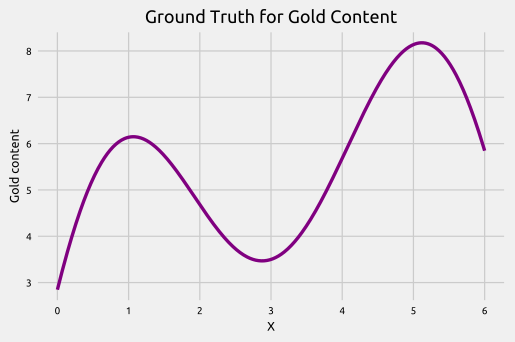
\includegraphics[height=.5\textheight]{bo-images/gifs/GT}
	\end{center}
\end{frame}

\begin{frame}{Surrogate Model}
	\urldef\matern\url{https://scikit-learn.org/stable/modules/generated/sklearn.gaussian_process.kernels.Matern.html}
	
	To model the unknown function we would use Gaussian Process Regressor. This is called the surrogate model.
	
	\begin{center}
		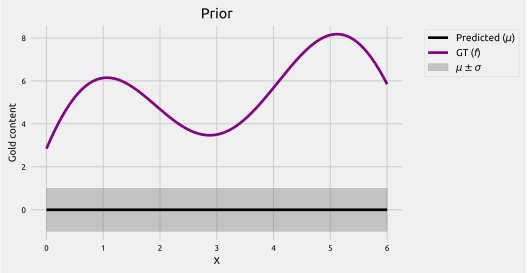
\includegraphics[height=.46\textheight]{bo-images/gifs/prior}
	\end{center}
	
	Initially the GP would not have any information, which can be seen by looking at the prior above. We assume that the gold distribution $f$ is smooth, via a Matern kernel \footnote{\matern}.
\end{frame}

\begin{frame}{Adding Training Data}
	\begin{center}
		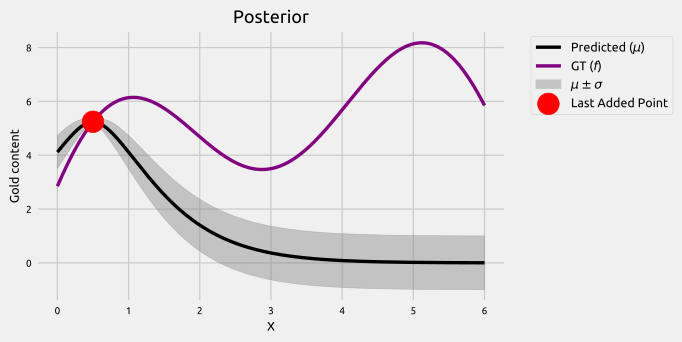
\includegraphics[height=.46\textheight]{bo-images/gifs/posterior}
	\end{center}
	
	We see how adding training point (drilling at a location and actually getting the gold concentration) changed the posterior of our surrogate model.
	
	We see that as more points are sampled, our surrogate is able to model more accurately.
\end{frame}

\section{Formalizing Bayesian Optimization}
\begin{frame}{Idea}
	Our main aim in the example discussed is to find the point where we can get the maximum gold content.
	
	Given this, it might be a good idea to use the information from the surrogate model. It might be likely where the surrogate predicts higher functional
	
	But, the surrogate is not a perfect model of $f$. Therefore, one would like to improve the surrogate model too. This is done by getting the functional values at points the surrogate is most uncertain about. This is \textbf{exploration}.
\end{frame} 

\begin{frame}
	
	\urldef\peter\url{https://www.youtube.com/watch?v=c4KKvyWW_Xk}
	
	Let us now formally introduce Bayesian Optimization. \footnote{Taken from \peter} Our goal is to find the $x$ where we reached global maximum (or minimum) of a function $f: \mathbb{R}^d \mapsto \mathbb{R}$.
\end{frame}

\begin{frame}
	We’d like to optimize $f: \mathbb{R}^d \mapsto \mathbb{R}$.
	
	\begin{itemize}
		\item $f$’s feasible set $A$ is simple, e.g., box constraints.
		
		\item $f$ is continuous but lacks special structure, e.g., concavity, that would make it easy to optimize.
		
		\item $f$ is derivative-free: evaluations do not give gradient information.
		
		\item $f$ is expensive to evaluate: the number of times we can evaluate it is severely limited.
		
		\item $f$ may be noisy. If noise is present, we’ll assume it is independent and normally distributed, with common but unknown variance.		
	\end{itemize}
\end{frame}

\begin{frame}
	Let us link the above constraints to our initial problem statement of gold mining.
	
	\begin{itemize}
		\item Our domain in the gold mining problem is a single-dimensional box constraint of $0 \leq x \leq 6$.
		
		\item Our ground truth can be seen as neither convex nor concave function, which resulted in local minima as well.
		
		\item Our evaluation (by drilling) of the amount of gold content at a location didn’t give us any gradient information.
		
		\item The function we used in the case of gold mining problem is extremely costly to evaluate (drilling costs millions).
		
		\item This constraint is still satisfied in our case as we had have taken noiseless measurements. Which can be considered as a Gaussian noise with zero mean and zero standard deviation.
	\end{itemize}

	We see that our original problem of mining gold fits into the criterions required to use BO.
\end{frame}

\begin{frame}{Acquisition Functions}
	\urldef\washu\url{https://www.cse.wustl.edu/~garnett/cse515t/spring_2015/files/lecture_notes/12.pdf}
	
	Original optimization problem $x^* = \text{argmax}_{x \in A} f(x)x$ is hard given the expensive nature of evaluating $f$.
	
	Idea: Replace original optimization into sequence of easier inexpensive optimizations on a function called acquisition function $(\alpha(x))$.
	
	Each optimization on $(\alpha(x))$ provides next point to get the functional value for. we can interpret the acquisition function as commensurate with how desirable evaluating $f$ at $x$ is expected to be for the maximisation problem. \footnote{Get more information at \washu}
\end{frame}

\begin{frame}{Combining Components}
	Let is re-wind and link all the things that we have discussed till now.
	
	\begin{enumerate}
		\item Choose a surrogate model and its prior over space of objectives $f$.
		
		\item Given the set of observations (function sampling), use Bayes rule to obtain the posterior.
		
		\item Use an acquisition function $\alpha(x)$, which is a function of the posterior to decide where to sample next $x_t = \text{argmax}_x \alpha(x)$.
		
		\item Add new sampled data to the set of observations and Goto Step \#2 till convergence or budget elapses.
	\end{enumerate}
\end{frame}

\begin{frame}{Core Ideas}
	We now have three core ideas associated with acquisition functions: 
	
	\begin{enumerate}
		\item They are a function of the surrogate posterior.
		
		\item They combine exploration and exploitation.
		
		\item They are inexpensive to evaluate.
	\end{enumerate}

	Let us now look into a few examples of commonly used acquisition functions to understand the concept better.
\end{frame}

\section{Acquisition Functions}
\begin{frame}{Probability of Improvement}
	Idea: Choose the next point as the one which has the highest probability of improvement over the current max $f(x^+)$, where $x^+ = \text{argmax}_{x_i \in x_{1:t}}f(x_i)$ and $x_i$ is the location queried at $i^{th}$ time step.
	
	Looking closely, we see PI is essentially the left tail probability of the posterior.
\end{frame}

\begin{frame}
	The formulation or procedure can be given as:
	
	\begin{itemize}
		\item Let $f(x^+)$ be the current highest value of the function.
		
		\item Let $\epsilon$ be close to zero.
		
		\item Choose $x_{t+1} = argmax(\alpha_{PI}(x))$ where $\alpha_{PI}(x) = P(f(x)) \geq (f(x^+) +\epsilon)$ 
	\end{itemize}
\end{frame}

\begin{frame}
	For the case where our surrogate is a GP, we can obtain a closed form solution making evaluation of $\alpha_{PI}$ cheap.
	$$x_{t+1} = argmax_x \Phi\left(\frac{\mu_t(x) - f(x^+) - \epsilon}{\sigma_t(x)}\right)$$
	where $\Phi(\cdot)$ indicates the CDF.
\end{frame}

\begin{frame}{Effects of $\epsilon$ in PI}
	\urldef\teaser\url{https://nipunbatra.github.io/distillpub/public/index.html\#Teaser1}
	
	PI makes use of $\epsilon$ in order to strike a balance between exploration and exploitation. Essentially by setting $\epsilon$ to some value, we want to choose a point such that the probability of improvement over $f(x^+) + \epsilon$ is the most.
	
	Increasing $\epsilon$ results in the locations with a larger $\sigma$ to benefit as their probability density is spread more. Thus points with more $\sigma$ would have a higher $\alpha_{PI}$ when the $\epsilon$ is set to a large value. \footnote{Have a look at \teaser \ for an interactive plot.}
\end{frame}

\forloop{iter}{0}{\value{iter} < 10}%
{%
	\begin{frame}{\theiter \ $|$ PI when $\epsilon = 0.01$}
		\begin{center}
			\includegraphics[width=\linewidth]{bo-images/pngs/PI/0.01/\theiter}
		\end{center}
	We see that having $\epsilon = 0.01$ primarily results in exploitation, and we are not able to get to the global maxima due to this myopic drilling point selection.
	\end{frame}
}

\forloop{iter}{0}{\value{iter} < 10}%
{%
	\begin{frame}{\theiter \ $|$ PI when $\epsilon = 1$}
		\begin{center}
			\includegraphics[width=\linewidth]{bo-images/pngs/PI/1/\theiter}
		\end{center}
	Looking above, we see increasing the value to $\epsilon = 1$, enables us to explore more and get near to the maximum value.
	\end{frame}
}

\forloop{iter}{0}{\value{iter} < 10}%
{%
	\begin{frame}{\theiter \ $|$ PI when $\epsilon = 8$}
		\begin{center}
			\includegraphics[width=\linewidth]{bo-images/pngs/PI/8/\theiter}
		\end{center}
		We see that we made things worse! Our model now uses $\epsilon = 8$, which has effectively resulted in way too much exploration. This amount of exploration is not able to exploit when we land somewhere near a global maximum.
	\end{frame}
}

\begin{frame}{Expected Improvement}
	Probability of improvement only looked at how likely is an improvement, but, shouldn’t we be looking into how much we can improve? The next criterion called, Expected Improvement, (EI) does exactly that!
\end{frame}

\begin{frame}
	In this acquisition function, $t + 1^{th}$ query point, $x_{t+1}$, is selected according to the equation below.
	$$x_{t+1} = argmin_x \mathbb{E} \left( ||h_{t+1}(x) - f(x^\star) || \ | \ \mathcal{D}_t \right)$$
	
	Where, $f$ is the actual ground truth function, $h_{t+1}$ is our GP posterior of the ground truth for $t+1^{th}$ timestep, $\mathcal{D}_t$ is the training data $\{(x_i, f(x_i))\} \ \forall x \in x_{1:t}$ and $x^\star$ is the actual position where the ground truth function takes the maximum value.
\end{frame}

\begin{frame}
	\urldef\doiMockus\url{https://doi.org/10.1007/BF00940509}
	
	In essence, we are trying to select the point that minimizes the distance to the objective evaluated at the maximum. Unfortunately, we don’t know the ground truth function, $f$. Mockus \footnote{Bayesian approach to global optimization and application to multiobjective and constrained problems
	\doiMockus}	proposed the following acquisition function to overcome the issue.
	$$x_{t+1} = argmax_x \mathbb{E} \left( {max} \{ 0, \ h_{t+1}(x) - f(x^+) \} \ | \ \mathcal{D}_t \right)$$
	
	Where $f(x^+)$ is the maximum value that has been encountered so far. 
\end{frame}

\begin{frame}
	For the case of the GP surrogate, the last equation can be easily converted to a closed form equation shown below.
	$$EI(x)= \begin{cases} (\mu_t(x) - f(x^+) - \epsilon)\Phi(Z) + \sigma_t(x)\phi(Z), & \text{if}\ \sigma_t(x) > 0 \\ 0 & \text{if}\ \sigma_t(x) = 0 \end{cases}$$
	
	where $\Phi(\cdot)$ indicates CDF and $\phi(\cdot)$ indicates pdf.
\end{frame}


\forloop{iter}{0}{\value{iter} < 10}%
{%
	\begin{frame}{\theiter \ $|$ EI when $\epsilon = 0.01$}
		\begin{center}
			\includegraphics[width=\linewidth]{bo-images/pngs/EI/0.01/\theiter}
		\end{center}
		We see that having $\epsilon = 0.01$ primarily results in exploitation, and we are not able to get to the global maxima due to this myopic drilling point selection.
	\end{frame}
}


\forloop{iter}{0}{\value{iter} < 10}%
{%
	\begin{frame}{\theiter \ $|$ EI when $\epsilon = 1.5$}
		\begin{center}
			\includegraphics[width=\linewidth]{bo-images/pngs/EI/1.5/\theiter}
		\end{center}
		As we expected, increasing the value to $\epsilon = 1.5$ makes the acquisition function explore more and exploit when the time comes. We see that it moves slowly once it reaches near the global maxima, trying to find the global maxima. In this case, the exploration is effectively helping us reach a higher functional value much earlier!
	\end{frame}
}


\forloop{iter}{0}{\value{iter} < 10}%
{%
	\begin{frame}{\theiter \ $|$ EI when $\epsilon = 3$}
		\begin{center}
			\includegraphics[width=\linewidth]{bo-images/pngs/EI/3/\theiter}
		\end{center}
		Is this better than before? Turns out a yes and a no. We see that here we do too much exploration given the value of $\epsilon = 3$. Which results in early reaching something close to global maxima, but unfortunately we don't exploit to get more gains near the global maxima.
	\end{frame}
}



















% [width=\linewidth]

%\begin{frame}{Bayes Rule - 2}
%\begin{itemize}
%	
%\item Test will produce 99\% true positive results for drug users and 99\% true negative results for non-drug users $\implies$
%\begin{itemize}
%	\item $P(Test=+|User=Drug) = 0.99$, or, $P(+|User) = 0.99$
%	\item and $P(-|\overline{User}) =0.99$ 
%\end{itemize}  
%		\item 0.5\% of people are users of the drug $\implies P(User) = 0.005$
%		\item Question: What is the probability that a randomly selected individual with a positive test is a drug user? $\implies P(User|+) = ?$
%		\item 
%				$P(User|+) = \frac{P(+|User)P(User)}{P(+)} = $
%		\item $\frac{P(\text{+}\mid\text{User}) P(\text{User})}{P(\text{+}\mid\text{User}) P(\text{User}) + P(\text{+}\mid\overline{User}) P(\overline{User})} = \frac{0.99\times 0.005}{0.99\times 0.005 + 0.01\times0.995} \approx .332$ 
%	
%\end{itemize}
%\end{frame}
%
%\begin{frame}{Another example on Bayes rule}
%\end{frame}
%
%
%\begin{frame}{Bayes Rule for Machine Learning}
%\begin{itemize}
%
%
%    \item $P(A|B)P(B) = P(B|A)P(A)$
%    \item Let us consider for a machine learning problem:
%    \begin{itemize}
%    	\item A = Parameters ($\theta$)
%    	\item B = Data ($\mathcal{D}$)
%    \end{itemize}
%\item We can rewrite the Bayes rule as:
%\begin{itemize}
%	\item $P(\theta|\mathcal{D}) = \frac{P(\mathcal{D}|\theta)P(\theta)}{P(\mathcal{D})}$
%	\item Posterior: 
%	\item Prior:
%	\item Likelihood
%	\item 
%\end{itemize}
%\end{itemize}
%\end{frame}
%
%\begin{frame}{Likelihood}
%\begin{itemize}
%	\item Likelihood is a function of $\theta$
%	\item Given a coin flip and 5 H and 1 T, what is more likely: P(H) = 0.5 or P(H) = 1
%\end{itemize}
%\end{frame}
%
%\begin{frame}{Bayesian Learning is well suited for online settings}
%content...
%\end{frame}
%
%\begin{frame}{Coin flipping}
%\begin{itemize}
%	\item Assume we do a coin flip multiple times and we get the following observation: \{H, H, H, H, H, H, T, T, T, T\}: 6 Heads and 4 Tails
%	\item  What is $P(Head)$?
%	\item Is your answer: 6/10. Why?
%\end{itemize}
%
%\end{frame}
%
%\begin{frame}{Coin flipping: Maximum Likelihood Estimate (MLE)}
%\begin{itemize}
%	\item We have $\mathcal{D} = \{\data_1, \data_2, ...\data_{N}\}$ for $N$ observations where each $\mathcal{D}_i \in \{H, T\}$
%	\item Assume we have $n_H$ heads and $n_T$ tails, $n_H + n_T = N$
%	\item Let us have $P(H) = \theta, P(T) = 1-\theta$
%	\item We have Likelihood, $L(\theta) = P(\mathcal{D}|\theta) = P(\data_1, \data_2, ..., \data_N|\theta)$
%	\item Since observations are i.i.d., $L(\theta) = P(\data_1|\theta).P(\data_2|\theta) ... P(\data_N|\theta)$
%\end{itemize}
%
%\end{frame}
%
%
%\begin{frame}{Coin flipping: Maximum Likelihood Estimate (MLE)}
%\begin{itemize}
%	\item  
%\begin{align*}  
%P(\data_i|\theta) =  \left
%\{\begin{array}{lr} \theta, & \text{for~} \data_i =H \\
%1-\theta, & \text{for~} \data_i = T
%\end{array}\right.\
%\end{align*}  
%\item Thus, $L(\theta) = \theta^{n_H}\times (1-\theta)^{n_T}$
%\item Log-Likelihood, $LL(\theta) = n_Hlog\theta + (n_T)(log(1-\theta))$
%\item $\frac{\partial LL(\theta)}{\partial \theta} = \frac{n_H}{\theta} - \frac{n_T}{1-\theta}$
%\item  For maxima, set derivative of LL to zero
%
%\item 	$\frac{n_H}{\theta} - \frac{n_T}{1-\theta} = 0 $
%\end{itemize}
%\begin{tcolorbox}
%	\begin{align*}
%	 \theta = \frac{n_H}{n_H + n_T}
%	\end{align*}
%
%\end{tcolorbox}
%Question: Is this maxima or minima?
%
%\end{frame}
%
%\begin{frame}{}
%\begin{align*}
%\frac{\partial^2 LL(\theta)}{\partial \theta^2} = \frac{-n_H}{\theta^2} + \frac{-n_T}{(1-\theta)^2} \in \mathbb R_-
%\end{align*}
%Thus, the solution is a maxima
%\end{frame}
%
%\begin{frame}{Maximum A Posteriori estimate (MAP)}
%\begin{itemize}
%
%
%\item \textbf{MLE does not handle prior knowledge}: What if we know that our coin is biased towards head?
%\item \textbf{MLE can overfit}: What is the probability of heads when we have observed 6 heads and 0 tails?
%\end{itemize}
%
%\end{frame}
%
%
%\begin{frame}{Maximum A Posteriori estimate (MAP)}
%Goal: Maximize the Posterior
%\begin{tcolorbox}
%	\begin{align}
%\hat{\theta}_{MAP} = \argmin_\theta P(\theta|\data)\\
%\hat{\theta}_{MAP}= \argmin_\theta P(\data|\theta)P(\theta)
%\end{align}
%\end{tcolorbox}
%
%\end{frame}
%
%\begin{frame}{Prior distributions}
%\end{frame}
%
%\begin{frame}{Beta Distribution}
%\end{frame}
%
%\begin{frame}{Beta Distribution}
%\end{frame}
%
%\begin{frame}{Coin toss: MAP estimate}
%\end{frame}
%
%\begin{frame}{Linear Regression: MLE}
%We previously saw 
%\begin{tcolorbox}
%\begin{align*}
%\hat{\theta}_{least-square} = \argmin_\theta \epsilon^T\epsilon = \argmin_\theta (y-X\theta)^T(y-X\theta)
%\end{align*}
%\end{tcolorbox}
%
%
%\end{frame}

\end{document}